\documentclass{article}
\usepackage{amsfonts}
\usepackage{hyperref}
\hypersetup{
    colorlinks=true,
    linkcolor=blue,
    filecolor=magenta,      
    urlcolor=cyan,
    pdftitle={Overleaf Example},
    pdfpagemode=FullScreen,
    }

\urlstyle{same}
\usepackage{graphicx} % Required for inserting images

\title{Exercise 2}
\author{Haim Lavi, 038712105}
\date{July 2025}

\begin{document}

\maketitle

\begin{enumerate}
    \item 
In time $t=0$, we have $X_0=B_1-(a+b0)B_{\frac{1}{1-0}}=B_1-aB_1=(1-a)B_1.$
But for $X_t$ to be a Brownian Motion, there must exist some constant $y\in\mathbb{R}$ (specifically $y=0$), such that a.s. $X_0=y$, but $(1-a)B_1$ is a random variable, not a constant. Unless $a=1$, and then a.s. ${X_0=B_1-1B_1=0}.$

Using ths identities $\mathbb{E}B_t^2=t$ and $\mathbb{E}B_tB_s=\min\{t,s\}$, we calculate

For $t<s$,
\[
\mathbb{E}(X_tX_s)=\mathbb{E}[(B_1-(a+bt)B_{\frac{1}{1-t}})(B_1-(a+bs)B_{\frac{1}{1-s}})=\]\[
=\mathbb{E}[B_1^2]-\mathbb{E}[(a+bt)B_\frac{1}{1-t}B_1]-\mathbb{E}[(a+bs)B_{\frac{1}{1-s}}B_1]+\mathbb{E}[(a+bt)(a+bs)B_{\frac{1}{1-t}}B_{\frac{1}{1-s}}]=
\]\[
=\mathbb{E}[B_1^2]-(a+bt)\mathbb{E}[B_\frac{1}{1-t}B_1]-(a+bs)\mathbb{E}[B_{\frac{1}{1-s}}B_1]+(a+bt)(a+bs)\mathbb{E}[B_{\frac{1}{1-t}}B_{\frac{1}{1-s}}]
\]
$0<t<s<1\Rightarrow{0<1-s<1-t<1}\Rightarrow{1<\frac{1}{1-t}<\frac{1}{1-s}}$, then
\[
=1-(a+bt)1-(a+bs)1+(a+bt)(a+bs)\frac{1}{1-t}=\]\[
=1-a-bt-a-bs+\frac{a^2+abt+abs+b^2ts}{1-t}=\]\[
=\frac{1-t-2a+2at-bt+bt^2-bs+bst+a^2+abt+abs+b^2ts}{1-t}
\]
But if $X_t$ and $X_s$ are Brownian Motion random variables, then $\mathbb{E}[X_tX_s]=\min\{t,s\}=t$\[\Rightarrow{1-t-2a+2at-bt+bt^2-bs+bst+a^2+abt+abs+b^2ts=t-t^2}\]
We collect all the constant expressions (expressions with only $a$ or $1$) to obtain $a^2-2a+1=0\Rightarrow{a=1}$, which we already saw. So we have $-t+2t-bt+bt^2-bs+bst+bt+bs+b^2ts-t+t^2=0\Rightarrow{bt^2+bst+b^2ts+t^2=0}$. We write the equations $bt^2+t^2=0$ and $b^2ts+bts=0$ to obtain $b=-1$.
So $X_t=B_1-(1-t)B_{\frac{1}{1-t}}$. We already saw that for $a=1$, a.s. $X_0=0$, and since it is a linear combination of $B_t$, it is also a.s continuous. $\mathbb{E}[X_{t+s}-X_t]=\mathbb{E}[B_1-(1-(t+s))B_{\frac{1}{1-t-s}}-[B_1-(1-t)B_{\frac{1}{1-t}}]]=\mathbb{E}[(1-t)B{\frac{1}{1-t}}]-\mathbb{E}[(1-(t+s)B_{\frac{1}{1-t-s}}]=(1-t)0-(1-(t+s))0=0$.

$var(X_{t+s}-X_t)=\mathbb{E}[(X_{t+s}-X_t)^2]-\mathbb{E}[X_{t+s}-X_t]^2=\mathbb{E}[(X_{t+s}-X_t)]^2]=\mathbb{E}[[(1-t)B_{\frac{1}{1-t}}-(1-(t+s))B_{\frac{1}{1-t-s}}]^2]=(1-t)^2\frac{1}{1-t}-2(1-t)(1-t-s)\frac{1}{1-t}+(1-t-s)^2\frac{1}{1-t-s}=1-t-2(1-t-s)+1-t-s=1-t-2+2t+2s+1-t-s=s$, so $X_{t+s}-X_t\sim{\mathcal{N}(0,s)}$.

\item Code can be found here: \url{https://github.com/HaimL76/ctmc2.git}

\begin{figure}[h]
\caption{Brownian Motion 35 different simulations}
\centering
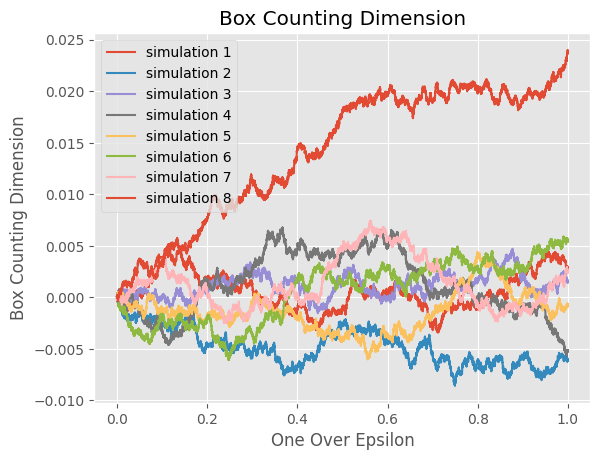
\includegraphics[width=0.5\textwidth]{brownian_motion_simulation.png}
\end{figure}
\begin{figure}[h]
\caption{Box Counting of the above simulations}
\centering
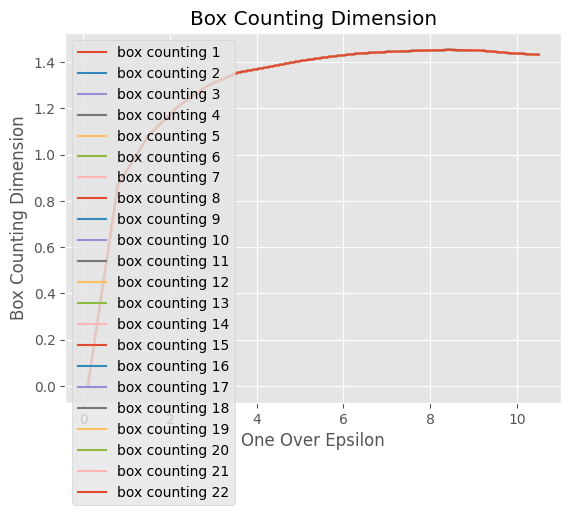
\includegraphics[width=0.5\textwidth]{box_counting_dimensions.png}
\end{figure}
We see that even though the 35 simulations go in different paths, the tendency of their box counting dimension around $1.4$ is very similar.

\item Code can be found here: \url{https://github.com/HaimL76/fbm.git}
We see that for the three different values of the Hurst parameter, the MSD stabilizes around the same value almost from the beginning of the time interval.
\begin{figure}[h]
\caption{Fractal Brownian Motion, Hurst=0.25}
\centering
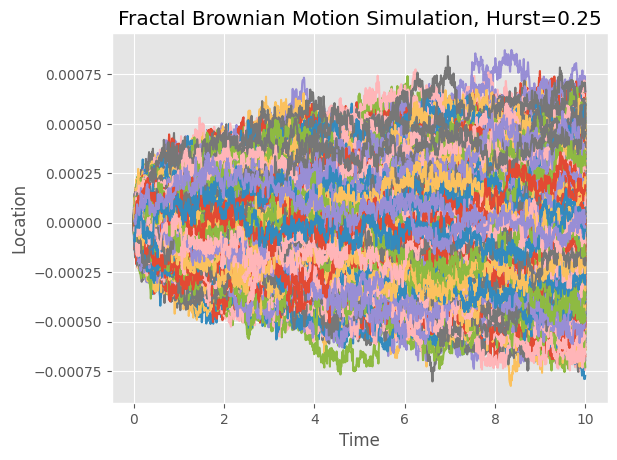
\includegraphics[width=0.5\textwidth]{fractal_brownian_motion_simulation_0.25.png}
\end{figure}
\begin{figure}[h]
\caption{Fractal Brownian Motion MSD, Hurst=0.25}
\centering
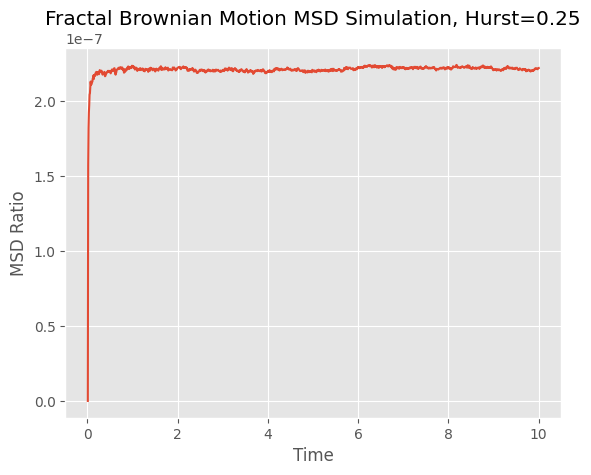
\includegraphics[width=0.5\textwidth]{fbm_msd_0.25.png}
\end{figure}
\begin{figure}[h]
\caption{Fractal Brownian Motion, Hurst=0.5}
\centering
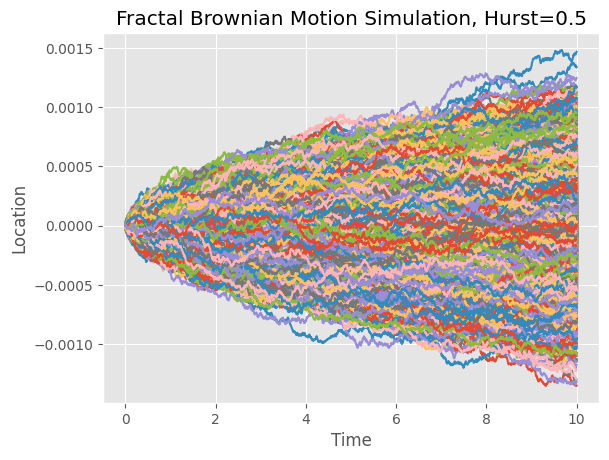
\includegraphics[width=0.5\textwidth]{fractal_brownian_motion_simulation_0.5.png}
\end{figure}
\begin{figure}[h]
\caption{Fractal Brownian Motion MSD, Hurst=0.5}
\centering
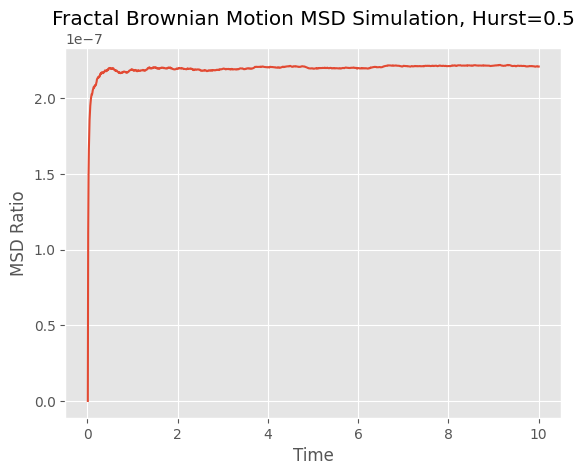
\includegraphics[width=0.5\textwidth]{fbm_msd_0.5.png}
\end{figure}
\begin{figure}[h]
\caption{Fractal Brownian Motion, Hurst=0.75}
\centering
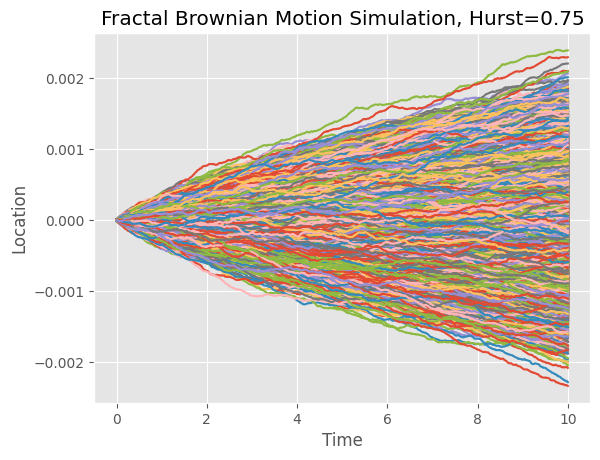
\includegraphics[width=0.5\textwidth]{fractal_brownian_motion_simulation_0.75.png}
\end{figure}
\begin{figure}[h]
\caption{Fractal Brownian Motion MSD, Hurst=0.75}
\centering
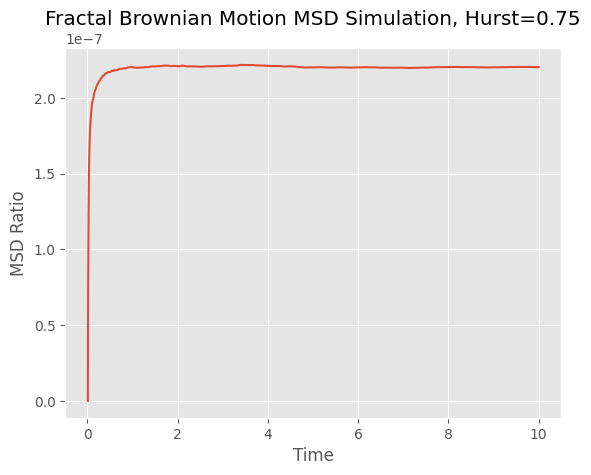
\includegraphics[width=0.5\textwidth]{fbm_msd_0.75.png}
\end{figure}
\end{enumerate}
\end{document}
